\chapter{Análise e Desenho da Solução}
\label{sec:3-Analise}

Depois de contextualizados os temas relevantes, o presente capítulo foca-se na análise do problema 
que sustenta este relatório e na apresentação do desenho da solução criada.

\section{Domínio do Problema}

O fluxo que trata da informação de catálogo é dos mais sensíveis e cruciais para o bom funcionamento
dos sistemas que integram os serviços do grupo Flutter. Este fluxo funciona em tempo-real recorrendo
ao uso de \textit{streams} para conseguir atingir este objetivo. Esta abordagem permite garantir
o processamento assíncrono dos dados relativos a este fluxo de uma forma otimizada.

De momento, os serviços responsáveis pelo processamento destes dados estão distribuídos em dois
\glspl{cluster} que usam \textit{Apache Storm} para a gestão do mesmo. Esta solução apresenta algumas
limitações passíveis de análise por forma a melhorar a capacidade de escalabilidade destes serviços. 

A primeira destas limitações é o elevado número de \ac{VM} presente em cada \gls{cluster}. Este 
problema impacta a solução na fase de lançamento de novas versões. Isto deve-se ao facto de toda a 
infraestrutura estar sob demanda constante com vários lançamentos paralelos de vários serviços em 
ao ser necessário criar novas \ac{VM} o processo responsável pela gestão de máquinas da
infraestrutura pode não ser capaz de responder ao pedido. Desta forma, diminuir o número de \ac{VM}
presentes no \gls{cluster} representaria uma melhoria na probabilidade da taxa de sucesso de
lançamento de uma nova versão (em todos os ambientes).

Além disso, existem topologias presentes em certos \glspl{cluster} que estão a usar um excesso de
recursos face aos recursos que necessitam para operar sem falhas em alturas de pico de utilização
dos mesmos.

\subsection{Contexto}

O grupo Flutter é uma das maiores empresas de apostas desportivas a nível mundial. Este grupo
possui várias marcas que operam em diferentes mercados, como o mercado britânico, australiano e
norte-americano. A empresa tem vindo a crescer de forma exponencial nos últimos anos e, como tal,
tem vindo a investir em novas tecnologias e a expandir a sua presença em novos mercados. No mercado
de \ac{UKI} o grupo Flutter adquiriu, nos últimos meses uma nova marca - \ac{SBG} \cite{skybet}. 
Esta aquisição requer que os serviços necessários para a operação da marca dentro da infraestrutura 
do grupo seja migrada para a mesma. De momento, o \textit{hardware} disponível nos \glspl{dc} da 
empresa não é capaz de suprir as necessidades de processamento necessária para hospedar estes 
serviços, logo, é necessário levar a cabo um processo de otimização de recursos nos \glspl{cluster} 
existentes de forma a tornar possível que o serviço opere sem falhas.

\subsection{Modelo de Domínio}

Nesta secção vai ser apresentado o \ac{MD} simplificado do fluxo de catálogo disponibilizado nas 
plataformas de \textit{sportsbook} das empresas do grupo Flutter. A compreensão deste modelo será
importante para acompanhar a solução apresentada de seguida. A Figura \ref{md} apresenta a vista
simplificada deste modelo.

\begin{figure}[H]
  \centerline{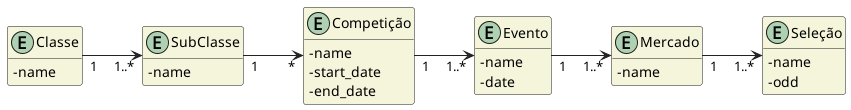
\includegraphics[scale=0.4]{media/content/analise/dm.png}}
  \caption{Modelo de Domínio - Fluxo de Catálogo (simplificado)}
  \label{md}
\end{figure}

De forma a ser mais simples acompanhar os termos apresentados na Figura \ref{md} vamos proceder 
a descrever uma hierarquia de exemplo:

\begin{itemize}
  \item \textbf{Classe} - Desporto (exemplo: Futebol)
  \item \textbf{SubClasse} - Especificação de Desporto (exemplo: Futebol Masculino)
  \item \textbf{Competição} - Competição (exemplo: Liga Portuguesa de Futebol)
  \item \textbf{Evento} - Evento (exemplo: FC Porto vs SC Espinho)
  \item \textbf{Mercado} - Tipo de Aposta (exemplo: Resultado Final)
  \item \textbf{Seleção} - Seleção de Aposta (exemplo: SC Espinho a vencer)
\end{itemize}

Como referido anteriormente, esta representação é apenas uma simplificação da realidade, isto
porque cada classe pode ter diferenças significativas na forma como representa a restante
hierarquia de relações entre entidades.

\section{Engenharia de Requisitos}

A Engenharia de Requisitos é uma área muito relevante no desenvolvimento de \textit{software}, pois 
sustenta a análise dos projetos, a primeira fase em que a equipa de desenvolvimento consegue 
compreender o domínio do negócio para o qual estão a desenvolver uma solução. Este passo representa 
o processo de obtenção de requisitos através de uma análise do problema e pressupõe a definição 
das necessidades, tanto por parte do cliente, como por necessidades técnicas, na procura de uma 
solução clara que valide a proposta apresentada. Seguindo um processo estruturado e adotando as 
melhores práticas, passamos a promover uma melhor comunicação entre as várias partes interessadas.

Considerando os aspetos mencionados, nesta secção serão apresentados os requisitos do sistema 
identificados e requisitados no início do projeto de maneira a garantir a que a solução desenvolvida 
vai de encontro com as necessidades apresentadas inicialmente. Estes requisitos podem ser 
categorizados em funcionais - funcionalidades distintas e essenciais que o sistema deve realizar, 
e não funcionais - restrições impostas para que o sistema realize os requisitos funcionais 
corretamente.

\subsection{Requisitos Não Funcionais}

Os requisitos não funcionais não se concentram no que o sistema faz, mas sim em como é esperado que
ele funcione. 

Os requisitos não funcionais apresentados em seguida, guiam-se pelo modelo FURPS+, um padrão de 
classificação qualitativa das características de um \textit{software} (\textbf{F}unctionality, 
\textbf{U}sability, \textbf{R}eliability, \textbf{P}erformance, \textbf{S}upportability), para uma 
melhor experiência do utilizador. O "\textbf{+}" refere-se a métodos de classificação diferentes, 
como por exemplo, restrições de design, implementação, interface ou físicos.

Estes requisitos são mais complexos de definir a nível do \gls{cluster}, pois cada topologia tem 
uma finalidade diferente, pelo que os requisitos são ligeiramente diferentes entre eles. De uma
forma geral, o sistema deve:

Para estes requisitos são definidos, para cada topologia, \acp{SLI} - os indicadores que mostram o
desempenho do sistema a todo o momento, \acp{SLO} - os objetivos que a equipa de desenvolvimento
deve atingir de forma a cumprir os \acp{SLA} - o acordo que o sistema mantém com os clientes a 
nível do seu funcionamento.

\vspace{5mm}

\textbf{Funcionalidade}
\begin{itemize}
  \item Encontram-se especificados na subsecção \nameref{sec:3-rf}.
\end{itemize}

\textbf{Usabilidade}
\begin{itemize}
  \item xxx
    \todo[inline]{Perguntar na Blip se há algum requisito enquadrado}
\end{itemize}

\textbf{Fiabilidade}

\begin{itemize}
  \item O sistema deve ser capaz de recuperar de falhas sem perda de dados.
  \item O sistema deve ser capaz de recuperar de falhas minimizando o tempo de inatividade.
  \item O sistema deve ser capaz de recuperar de falhas sem intervenção manual.
\end{itemize}


\textbf{Desempenho}
\begin{itemize}
  \item O sistema deve manter a capacidade de processamento que tinha antes da intervenção.
  \item O sistema deve ser capaz de processar transações em dia de pico de catálogo sem atrasos 
    significativos na latência.
  \item O sistema deve ser capaz de processar transações em dia de pico de catálogo minimizando o 
    tempo de resposta.
\end{itemize}

\textbf{Suporte}
\begin{itemize}
  \item xxx
    \todo[inline]{Perguntar na Blip se há algum requisito enquadrado}
\end{itemize}

\textbf{Restrições de Design}
\begin{itemize}
  \item O sistema deve suportar quatro ambientes - \ac{QA}, desenvolvimento, 
    performance e produção.
  \item O sistema deve estar replicado em dois \glspl{dc}.
  \item Todas as \ac{VM} do mesmo \gls{cluster} devem ter o mesmo \gls{flavour}.
  \item A paralelização deve ser feita por \ac{VM} e não por processo. Ou seja, a mesma \ac{VM} 
    não pode ter dois processos a correr em paralelo.
\end{itemize}

\subsection{Requisitos Funcionais}
\label{sec:3-rf}

Os requisitos funcionais especificam as unidades funcionais de um sistema de \textit{software}.
Estes requisitos concentram-se nas funções que devem ser disponibilizadas, descrevem as
funcionalidades, comportamentos e operações específicas que os utilizadores devem ser capazes de 
executar, podendo variar desde ações básicas, como entrada e saída de dados, a algoritmos 
específicos e processos de negócio.

De forma a facilitar a compreensão dos requisitos funcionais estes encontram-se descritos na 
Tabela \ref{tab:reqfun} e na Figura \ref{dcu}, na forma de \textit{User Stories}, seguindo a 
estrutura apresentada no artigo "(User) Stories for Analytics Projects - Part 1". \cite{us}.

% \begin{table}[H]
%   \begin{center}
%     \caption{Requisitos Funcionais}
%     \vspace{5mm}
%     \label{tab:reqfun}
%     \begin{tabular}{|c|l|}
%       \hline
%       ID & User Story                                                                  \\ \hline
%       1  & \begin{tabular}[c]{@{}l@{}}Como Engenheiro de Aplicações, pretendo que seja efetuado \\
%         um estudo que determine possíveis otimizações de recursos nos \glspl{cluster} dos serviços \\
%       de catálogo .\end{tabular} \\ \hline
%       2  & \begin{tabular}[c]{@{}l@{}}Como Engenheiro de Aplicações, pretendo que seja elaborado \\
%         um plano que defina como serão efetuadas as alterações nos recursos dos \glspl{cluster} \\
%         dos serviços de catálogo .\end{tabular} \\ \hline
%       3  & \begin{tabular}[c]{@{}l@{}}Como Engenheiro de Aplicações, pretendo que sejam efetuadas \\
%       reduções de recursos nos \glspl{cluster} dos serviços de catálogo atuais.\end{tabular} \\ \hline
%       4  & \begin{tabular}[c]{@{}l@{}}Como Engenheiro de Aplicações, pretendo que a versão de \\
%         \textit{Apache Storm} utilizada pelos \glspl{cluster} dos serviços de catálogo seja atualizada \\
%         para a versão mais recente.\end{tabular} \\ \hline
%       5  & \begin{tabular}[c]{@{}l@{}}Como XXX, quero XXX.\end{tabular} \\ \hline
%     \end{tabular}
%   \end{center}
% \end{table}

\begin{table}[H]
  \begin{center}
    \caption{Requisitos Funcionais}
    \vspace{5mm}
    \label{tab:reqfun}
    \begin{tabular}{|c|l|}
      \hline
      ID & User Story                                                                  \\ \hline
      1  & \begin{tabular}[c]{@{}l@{}}Como utilizador, pretendo consultar os eventos ativos \\
        num determinado dia. \\
      \end{tabular} \\ \hline
        2  & \begin{tabular}[c]{@{}l@{}}Como utilizador, pretendo consultar os tipos de aposta \\
        disponíveis para um determinado evento. \\
      \end{tabular} \\ \hline
        3  & \begin{tabular}[c]{@{}l@{}}Como utilizador, pretendo consultar as \glspl{odd} de um\\
        num determinado evento. \\
      \end{tabular} \\ \hline
    \end{tabular}
  \end{center}
\end{table}

\begin{figure}[H]
  \centerline{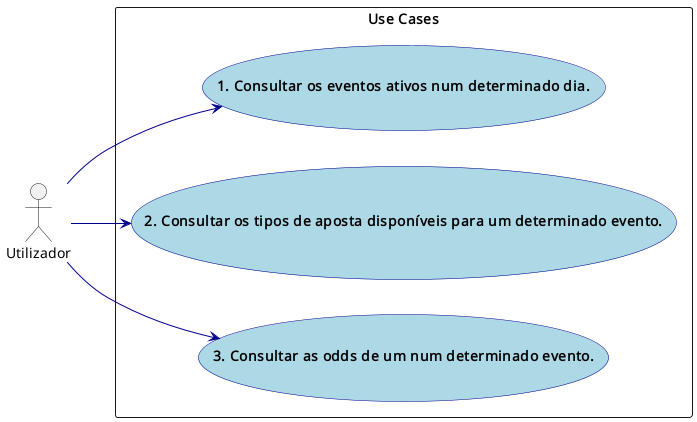
\includegraphics[scale=0.4]{media/content/analise/ucd.png}}
  \caption{Diagrama de Casos de Uso}
  \label{dcu}
\end{figure}

\section{Desenho da Solução}

Após a análise do problema definido juntamente com os requisitos funcionais e não funcionais,
apresentados anteriormente, o objetivo desta secção é documentar as fases que fazem parte do
desenho da solução idealizada.

Desta forma, se for possível alterar o \gls{flavour} destes \glspl{cluster} vai ser possível economizar
recursos. Para atingir este objetivo existem várias abordagens possíveis, como por exemplo, a
alteração do número de \ac{VM} presentes em cada \gls{cluster}, a alteração do \gls{flavour}
de cada \gls{cluster} ou a alteração da distribuição de serviços por \gls{cluster}.

\subsection{Análise de Uso de Recursos}

A primeira fase do desenho da solução passa pela análise do uso de recursos dos \glspl{cluster}
que suportam os serviços de catálogo. Para tal, foram analisadas duas janelas temporais distintas
onde os serviços sofreram uma carga acima do normal. Desta forma, é possível ter uma visão clara
das possíveis otimizações de recursos a fazer já que o objetivo final é que o \gls{cluster}
mantenha a sua capacidade de processamento e seja capaz de suportar a mesma carga a que estava
sujeito antes desta intervenção.

Para isso, é importante, em primeiro lugar, compreender a forma como estes serviços são requisitados
pelo sistema para, desta forma, ser possível analisar o intervalo de datas correto. Neste caso,
todos os serviços disponibilizados pelos \glspl{cluster} são relativos ao catálogo, ou seja,
à informação relativa aos vários eventos disponibilizados aos clientes. Desta forma, os intervalos
a analisar devem ser períodos em que sejam criados muitos eventos novos, ou momentos em que
estejam a ser realizados vários eventos em simultâneo e o sistema de atualização de \glspl{odd}
esteja a ser bastante utilizado.

Após discussão com vários elementos mais experientes no negócio concluiu-se que os intervalos
adequados a esta análise seriam em agosto - quando são criados os eventos relacionados com as
principais ligas dos maiores desportos a nível europeu, como futebol e basquetebol - e dezembro 
quando existe uma nova vaga de criação de eventos nesses desportos e também a disponibilização 
dos calendários noutros desportos disponíveis nas plataformas de \textit{sportsbook} como
corridas de cavalos.

Para a análise destes dados foram usadas as métricas disponibilizadas no \textit{Grafana}. Em alguns
casos foi necessário a criação de novos \textit{dashboards} para a análise de métricas mais 
específicas para cada serviço, mas na maioria dos casos as métricas mais relevantes eram métricas 
de sistema, como uso de processador e de memória RAM.

Esta análise foca-se no uso de recursos de cada topologia. Na Figura \ref{analise-ofs} podemos
analisar o uso de recursos de um dos \glspl{cluster}. A restante análise encontra-se
presente em no Anexo \ref{appendix-a}.

\begin{figure}[H]
  \centerline{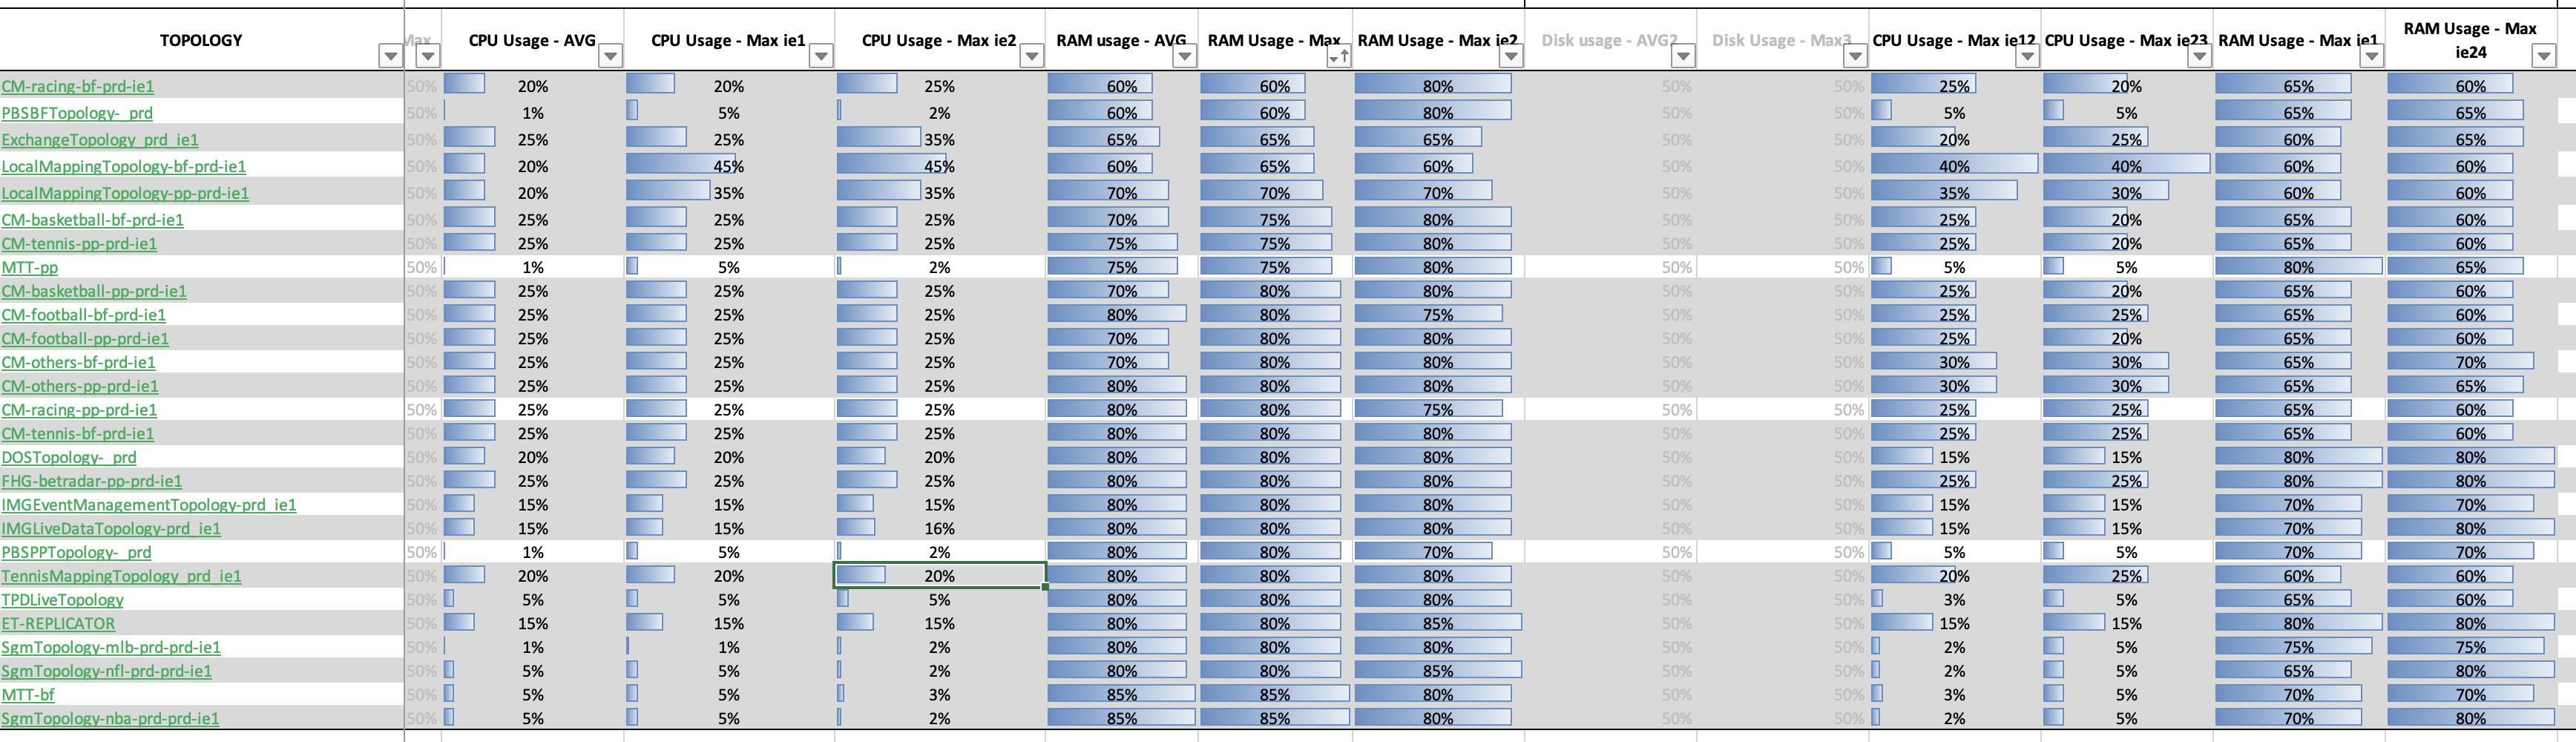
\includegraphics[scale=0.25]{media/content/analise/analise-ofs.png}}
  \caption{Análise do uso de recursos de um dos \textit{clusters}}
  \label{analise-ofs}
\end{figure}

Esta análise permitiu concluir que existem topologias que estão hospedadas num \gls{cluster}
com um \gls{flavour} superior ao que necessitam para processar a carga que lhes é atribuída,
mesmo em momentos de pico. 

\subsection{Possíveis abordagens}

Após concluída esta fase de análise foi possível sugerir novas abordagens para a distribuição
das topologias pelos \glspl{cluster} de forma a otimizar o uso total de recursos dos mesmos.

Para isso foram criadas três abordagens alternativas que tentam resolver este problema. Todas estas
abordagens vão ser analisadas e discutidas de forma a ser possível compreender qual o motivo da
escolha da alternativa que foi optada internamente.

A distribuição das topologias pelos \glspl{cluster} é apresentada, de seguida, em formato de 
tabela onde, em cada coluna é representado um \gls{cluster}, ou \ac{TLA}, como é referido 
internamente no contexto da empresa, e o respetivo \gls{flavour}. Em cada uma das células é
apresentada uma topologia e um multiplicador, por exemplo, \textit{ELR*2}. As letras são uma 
abreviatura do nome da topologia e o multiplicador refere-se à quantidade de diferentes
implementações da topologia a serem executadas no \gls{cluster}. Este multiplicador não representa
o fator de replicação da topologia, mas sim várias instâncias com implementações diferentes, por
exemplo, algumas topologias devem ter implementações diferentes por marca - topologias
\textit{brand-aware} - algumas precisam de diferentes implementações por desporto, por exemplo,
implementações diferentes para futebol e ténis.

No fim de cada tabela temos a quantidade de recursos (número de \ac{CPU} e GB de RAM) que cada 
configuração de topologias vai usar no total.

\subsubsection{Alternativa 1}

A primeira alternativa, representada na Figura \ref{proposal-1}, serve de base para todas as
alternativas que serão analisadas subsequentemente. A ideia é criar um novo \gls{cluster}
para receber as topologias que não necessitam de tanta capacidade computacional associado. Desta 
forma, será possível libertar os restantes \glspl{cluster} do número excessivo de \ac{VM} 
e, ao reduzir os \glspl{flavour} de todas as \ac{VM} procedemos à redução do uso total do
conjunto, pois é efetuada a transição de um conjunto de \ac{VM} com uma especificação, por exemplo,
4 \ac{CPU} e 12GB de memória RAM para um conjunto de \ac{VM} com 2 \ac{CPU} e 10GB RAM. No exemplo
anterior, assumindo um \gls{cluster} com 100 máquinas, teriamos uma redução de 50 \ac{CPU} e 20GB 
de RAM.

\begin{figure}[H]
  \centerline{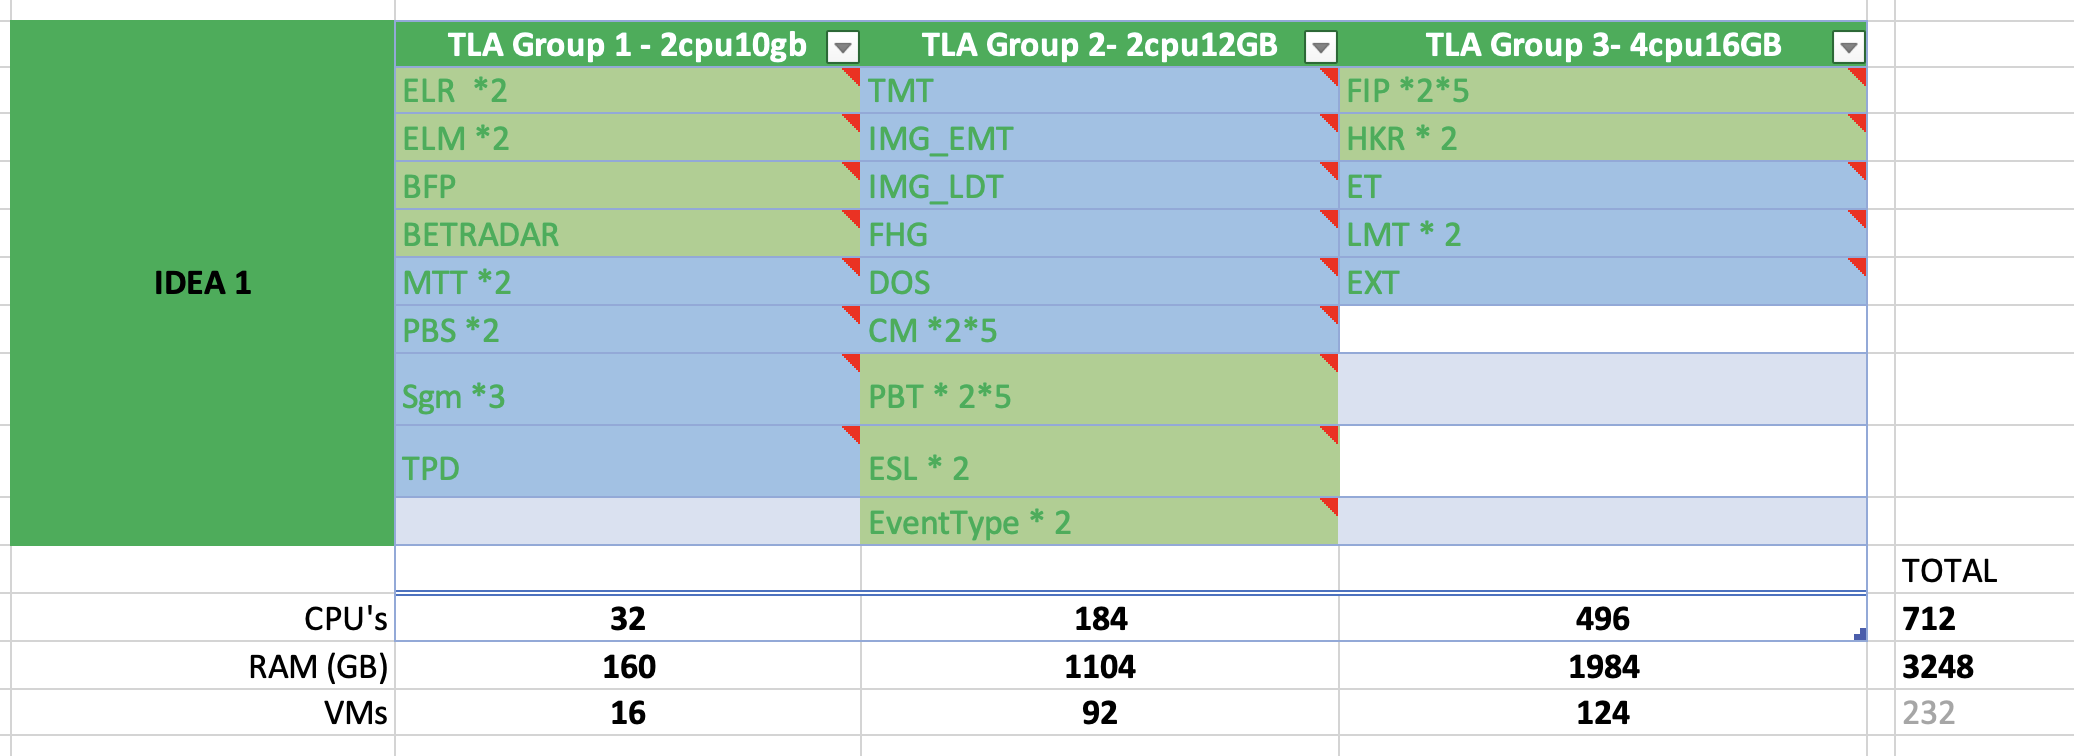
\includegraphics[scale=0.4]{media/content/analise/proposal-1.png}}
  \caption{Distribuição de topologias pelos \textit{clusters} - Alternativa 1}
  \label{proposal-1}
\end{figure}

\subsubsection{Alternativa 2}

A segunda alternativa, representada na Figura \ref{proposal-2}, diminui a memória RAM utilizada no
primeiro \gls{cluster}, além de reformular a organização das topologias pelos restantes. 

O número de \ac{VM} hospedadas no mesmo \gls{cluster} não deve ser demasiado elevado de forma a
evitar uma carga demasiado elevada no processo de implantação, isto porque, devido à forma como 
funciona o \textit{Apache Storm} a alteração numa topologia implica o processo de implantação de
todo o \gls{cluster} e, logicamente, quanto maior a quantidade de \ac{VM} que devem ser criadas
durante o processo, mais demorado se tornará.

\begin{figure}[H]
  \centerline{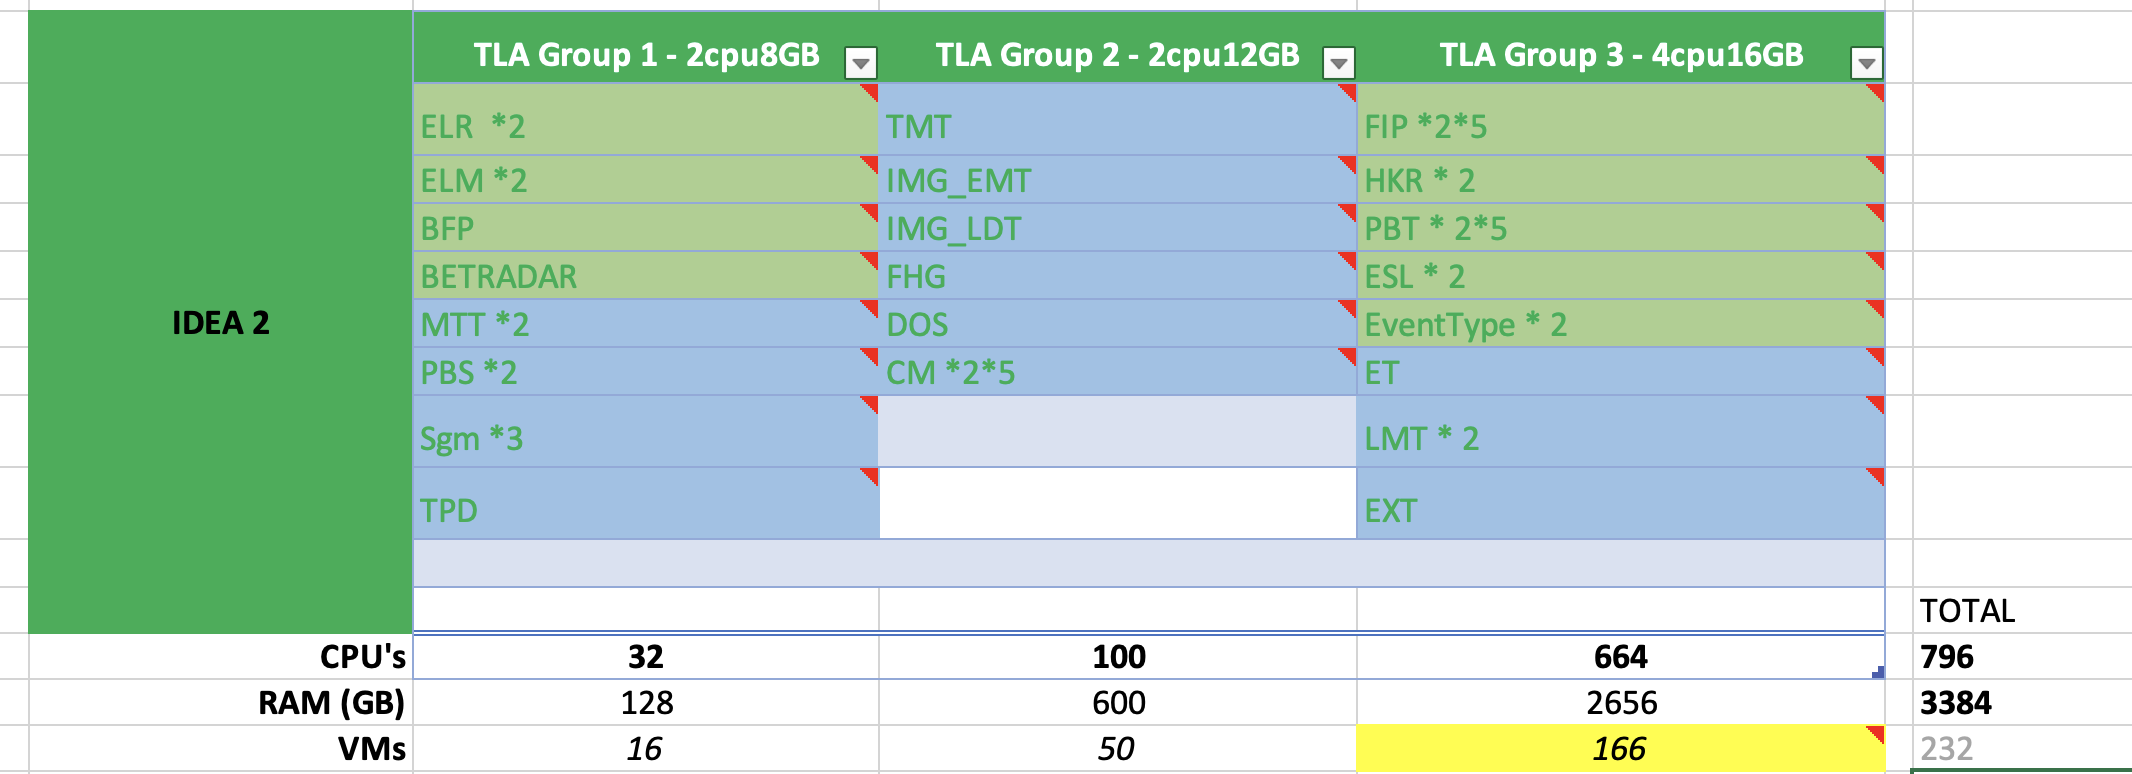
\includegraphics[scale=0.4]{media/content/analise/proposal-2.png}}
  \caption{Distribuição de topologias pelos \textit{clusters} - Alternativa 2}
  \label{proposal-2}
\end{figure}

Esta abordagem acaba por ser inferior às restantes por duas questões - o tamanho, em termos de número 
de \ac{VM}, do terceiro \gls{cluster} e a quantidade total de recursos superior à proposta
analisada anteriormente.

\subsubsection{Alternativa 3}

A terceira, e última, alternativa analisada acaba por ser a mais vantajosa em quase todos os 
aspetos, mas acabou por ser descartada devido após análise por parte das equipas que desenvolvem as 
topologias. Isto porque uma das topologias é uma exceção às restantes no sentido em que todas as
restantes, como mencionado anteriormente, a paralelização só é permitida ser efetuada por máquina, 
ou seja, a mesma máquina não pode correr mais que um processo da topologia, paralelamente.
Devido à necessidade acima do normal de paralelização por parte desta topologia em específico
acabou por ser aberta a exceção e neste caso cada máquina corre dois processos em paralelo.
Desta forma, a análise efetuada anteriormente não pode ser interpretada da mesma forma para esta
topologia, o que invalida esta alternativa.

\begin{figure}[H]
  \centerline{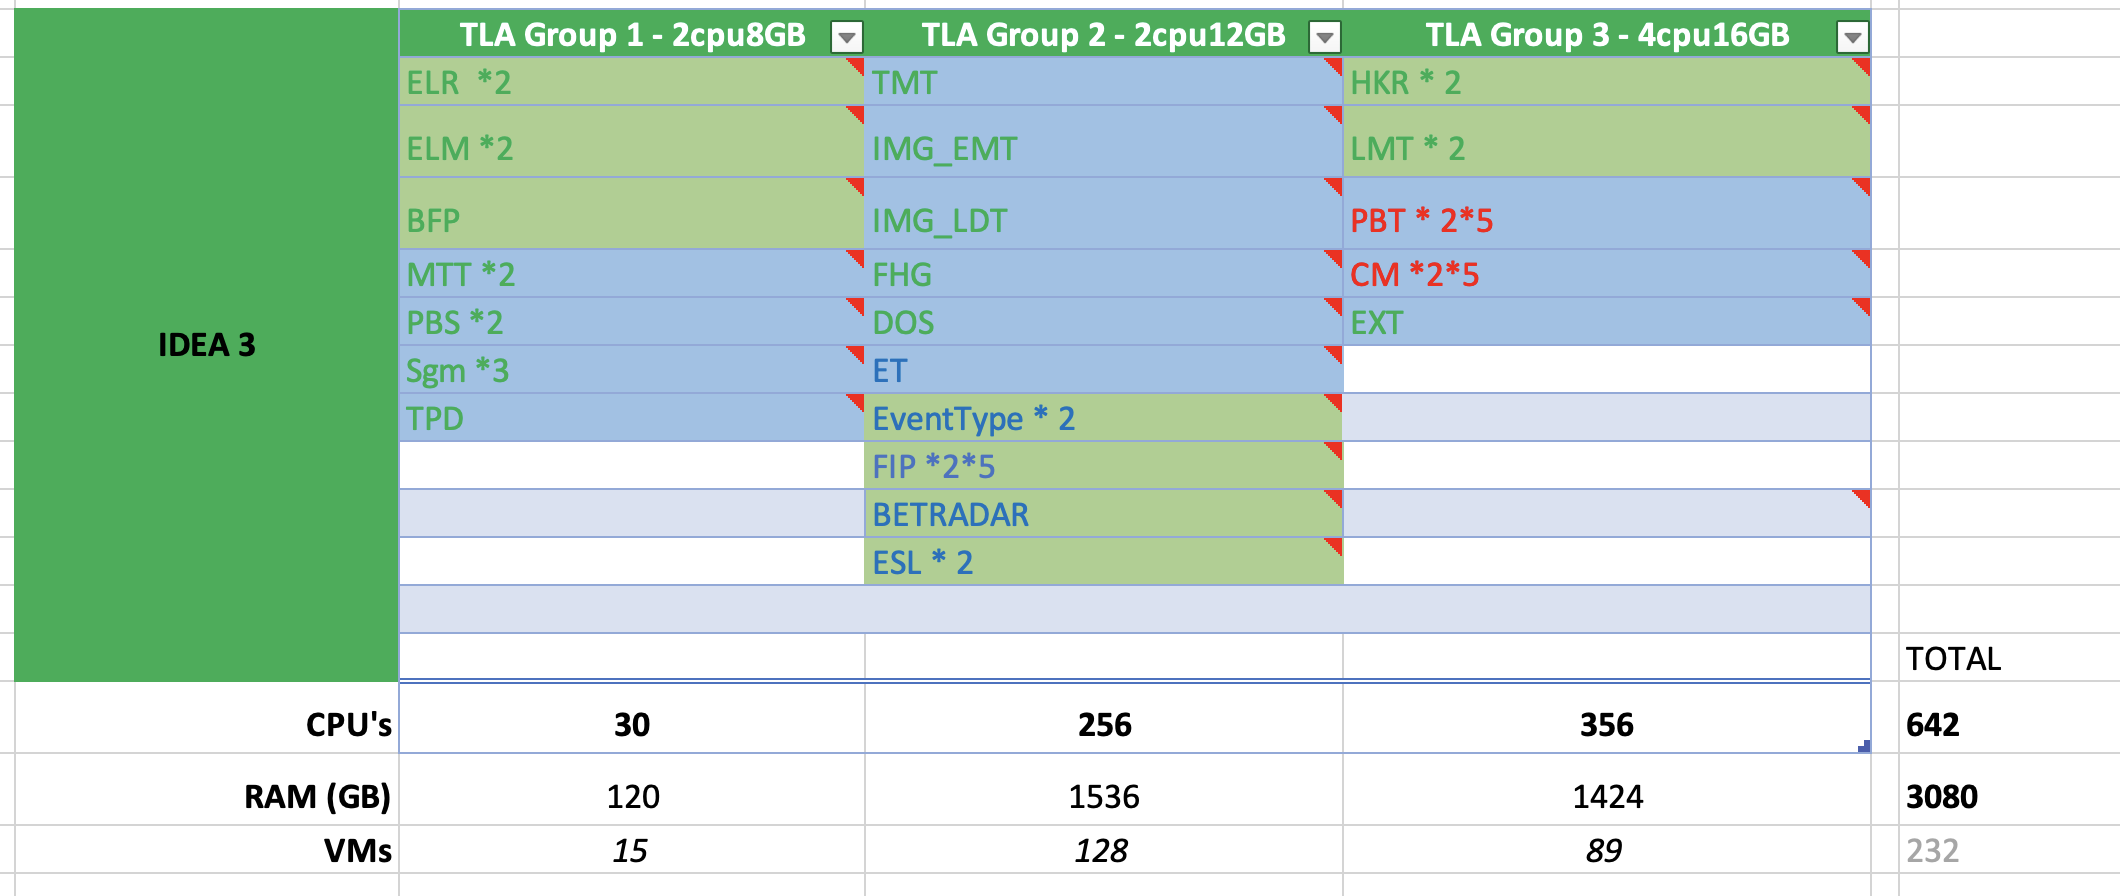
\includegraphics[scale=0.4]{media/content/analise/proposal-3.png}}
  \caption{Distribuição de topologias pelos \textit{clusters} - Alternativa 3}
  \label{proposal-3}
\end{figure}

\subsubsection{Comparação entre alternativas}

Após uma análise cuidada de todas estas alternativas acabou por ser escolhida a primeira alternativa
com a alteração da memória RAM do primeiro \gls{cluster} chegando à opção ilustrada na Figura
\ref{proposal-final}.

\begin{figure}[H]
  \centerline{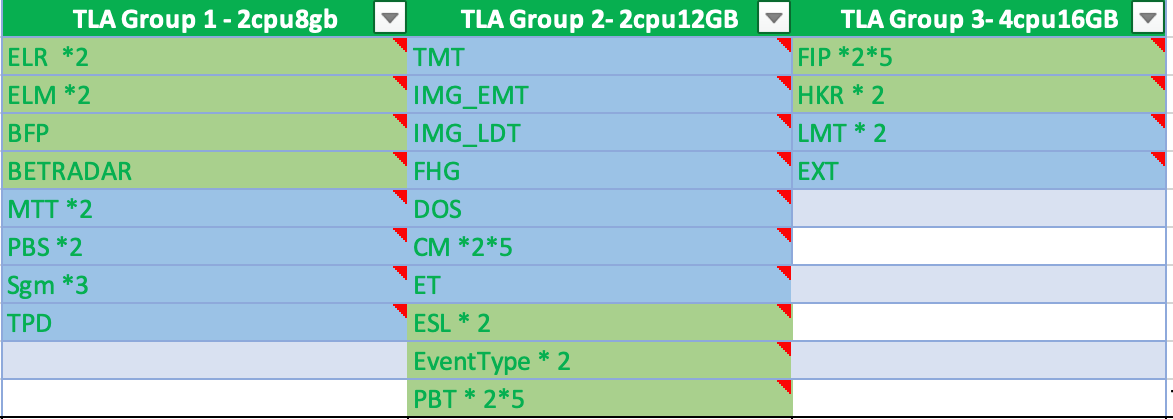
\includegraphics[scale=0.6]{media/content/analise/proposal-final.png}}
  \caption{Distribuição de topologias pelos \textit{clusters} - Alternativa Final}
  \label{proposal-final}
\end{figure}

Podemos observar na Figura \ref{comparison-proposal} a comparação entre todas as propostas
analisadas em termos de uso total de recursos em todos os ambientes.

\begin{figure}[H]
  \centerline{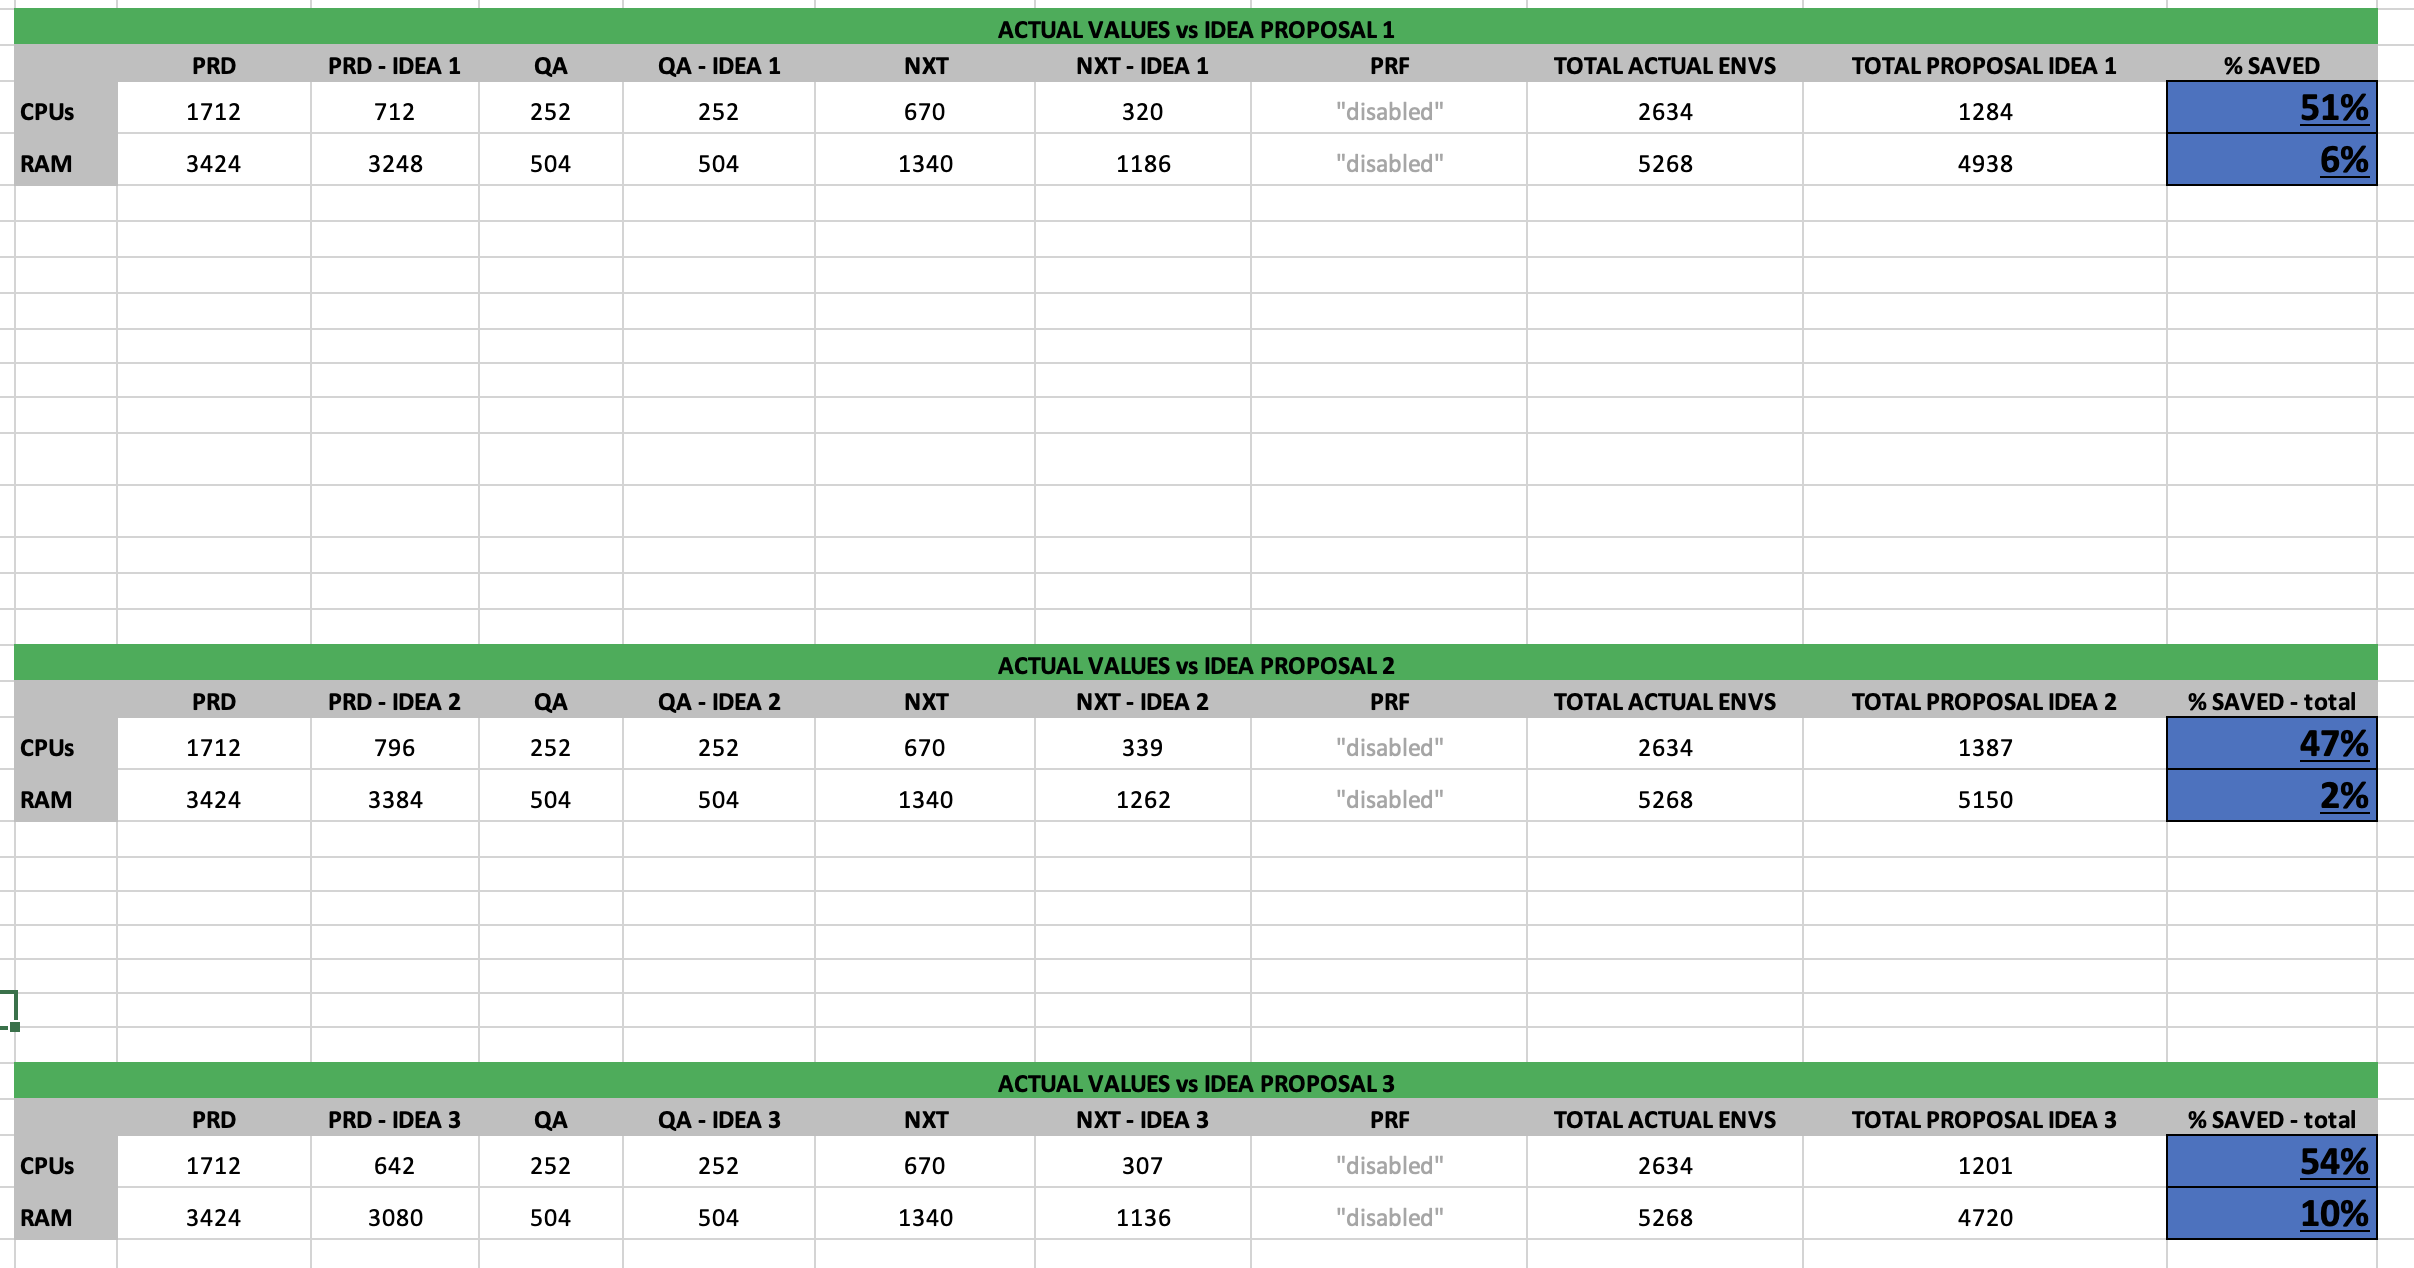
\includegraphics[scale=0.4]{media/content/analise/proposal-comparison.png}}
  \caption{Comparação de propostas de atualização}
  \label{comparison-proposal}
\end{figure}

\subsection{Processo de implantação}

Após decidir qual a abordagem a ser seguida é necessário definir o processo de implantação a ser
seguido. Este processo deve ser claro e conciso de forma a garantir que todas as equipas envolvidas
compreendam o processo que vai ser implementado e, desta forma, maximizar a probabilidade de
sucesso da intervenção. 

Este processo foi dividido em três passos que vão ser descritos e analisados de seguida. Por uma
questão de simplicidade no trabalho de análise, todos os quadros apresentados de seguida têm por 
base apenas os valores de recursos dos ambientes de produção, ou seja, para obter os valores reais
de redução de recursos deve ser necessário ainda ter em conta os recursos dos restantes ambientes
e multiplicar todos os resultados por dois já que todas as alterações devem ser replicadas em 
ambos os \glspl{dc}. Esta simplificação foi feita já que todas estas variáveis adicionais podem 
ser desprezadas dadas as semelhanças entre ambientes e a dimensão total da infraestrutura em
análise.

Na Figura \ref{strat-current} podemos observar o estado atual dos \glspl{cluster}. Este é o ponto
de partida para esta intervenção. 

\begin{figure}[H]
  \centerline{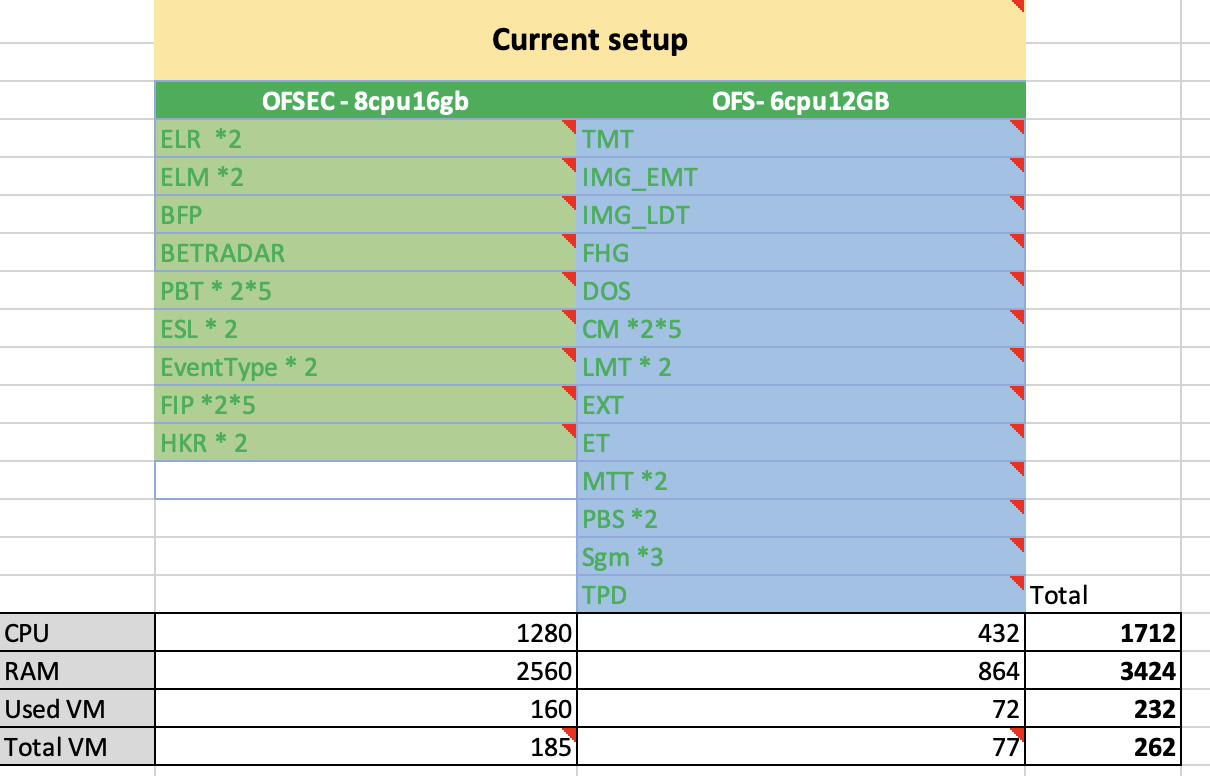
\includegraphics[scale=0.5]{media/content/analise/strat-current.png}}
  \caption{Processo de implantação - Estado atual}
  \label{strat-current}
\end{figure}

No primeiro passo, representado na Figura \ref{strat-1}, é efetuada uma redução de recursos 
de ambos os \glspl{cluster}. Esta redução parte do princípio de que, sendo possível obter a 
solução final apresentada anteriormente, então, por definição, as topologias devem ser capazes de
operar sem problemas usando estes novos \glspl{flavour}. Esta intervenção só por si, representa
46\% de redução no uso total de \ac{CPU} (no ambiente de produção).

\begin{figure}[H]
  \centerline{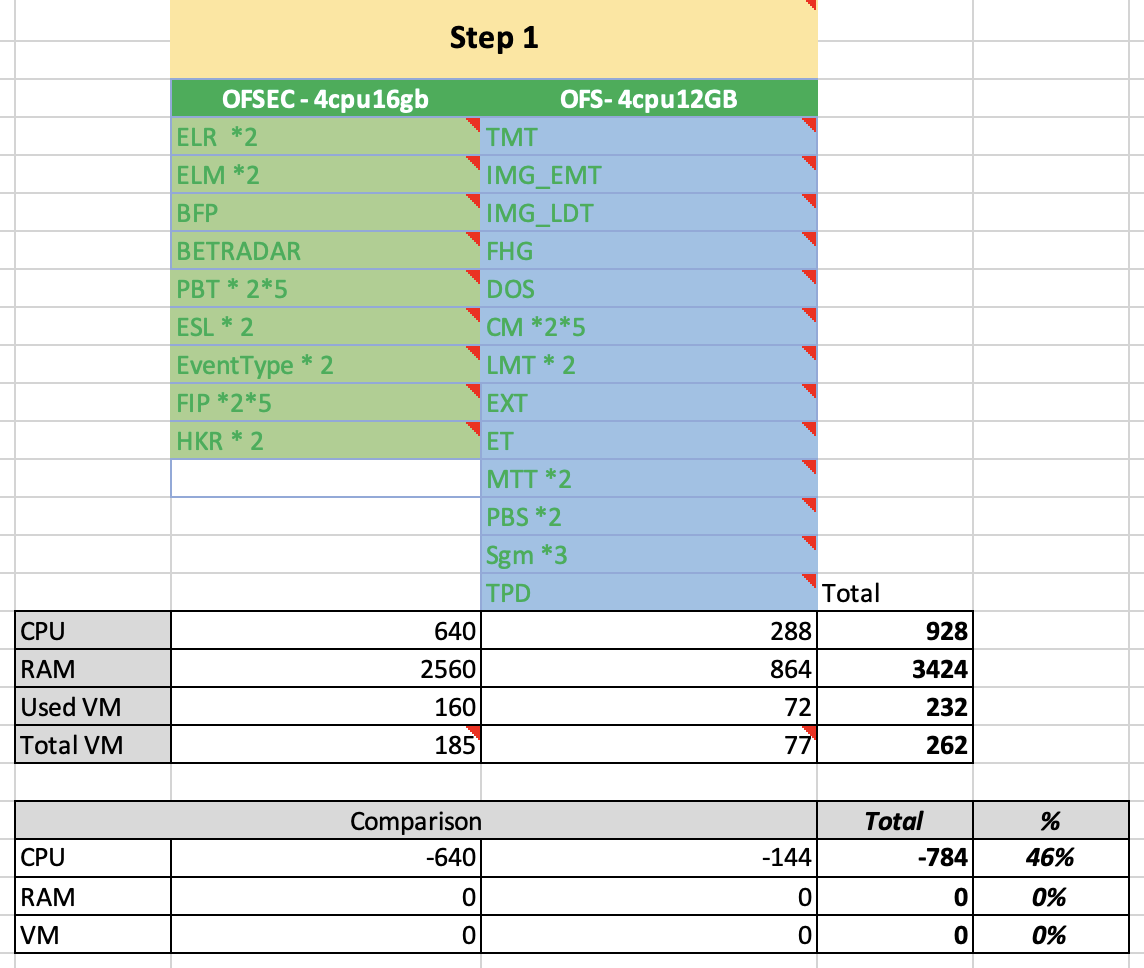
\includegraphics[scale=0.5]{media/content/analise/strat-1.png}}
  \caption{Processo de implantação - Passo 1}
  \label{strat-1}
\end{figure}

O segundo passo foi dividido em duas etapas - a criação do novo \gls{cluster}, representado na 
Figura \ref{strat-2} e a migração das topologias entre \glspl{cluster} (Figura \ref{strat-2_1}).

\begin{figure}[H]
  \centerline{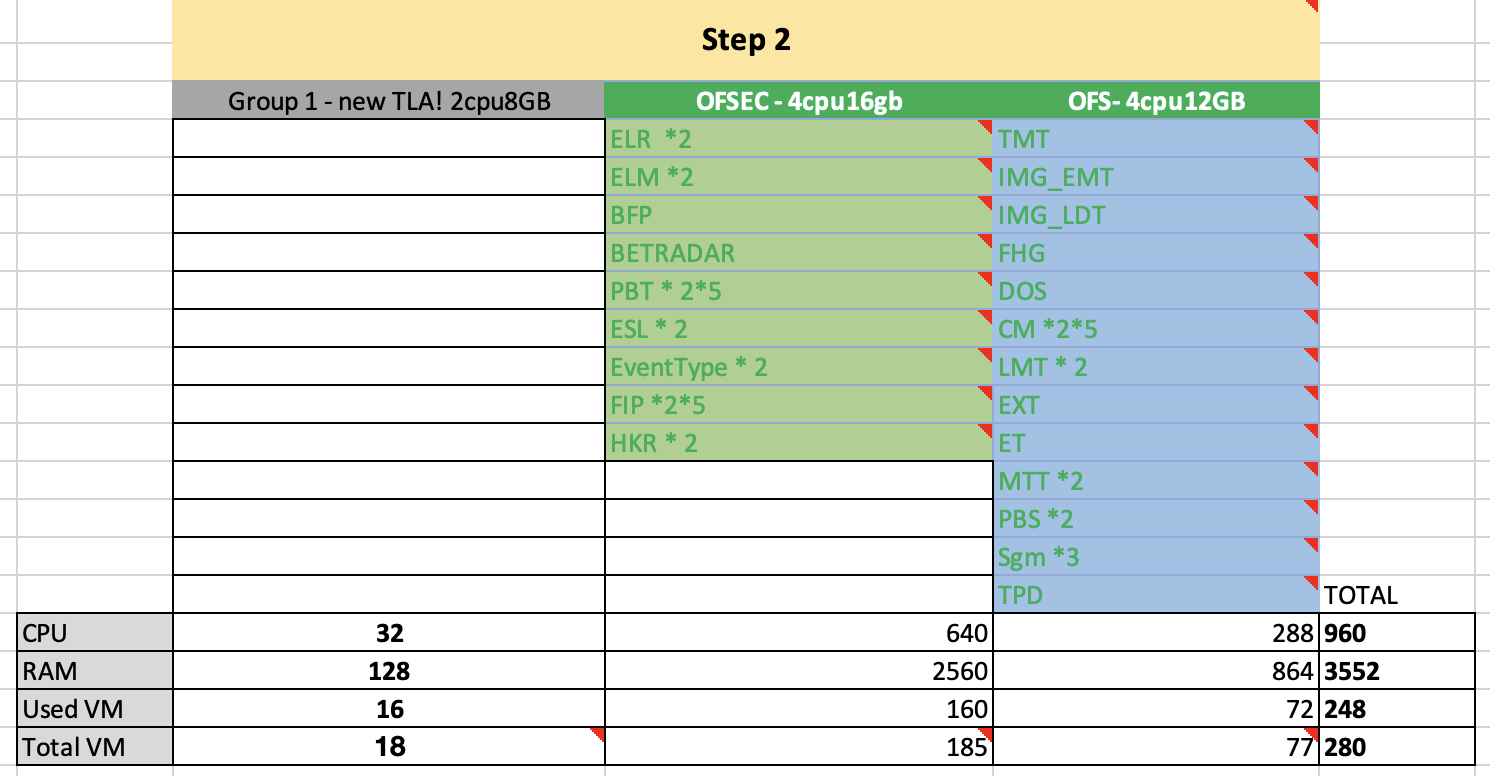
\includegraphics[scale=0.5]{media/content/analise/strat-2.png}}
  \caption{Processo de implantação - Passo 2}
  \label{strat-2}
\end{figure}

A segunda etapa deste passo é a etapa mais crítica de todo o processo, isto porque, nesta fase, é
crucial ter a total compreensão dos processos de replicação e \gls{failover} de cada topologia de
forma a minimizar o tempo de indisponibilidade de cada serviço.

\begin{figure}[H]
  \centerline{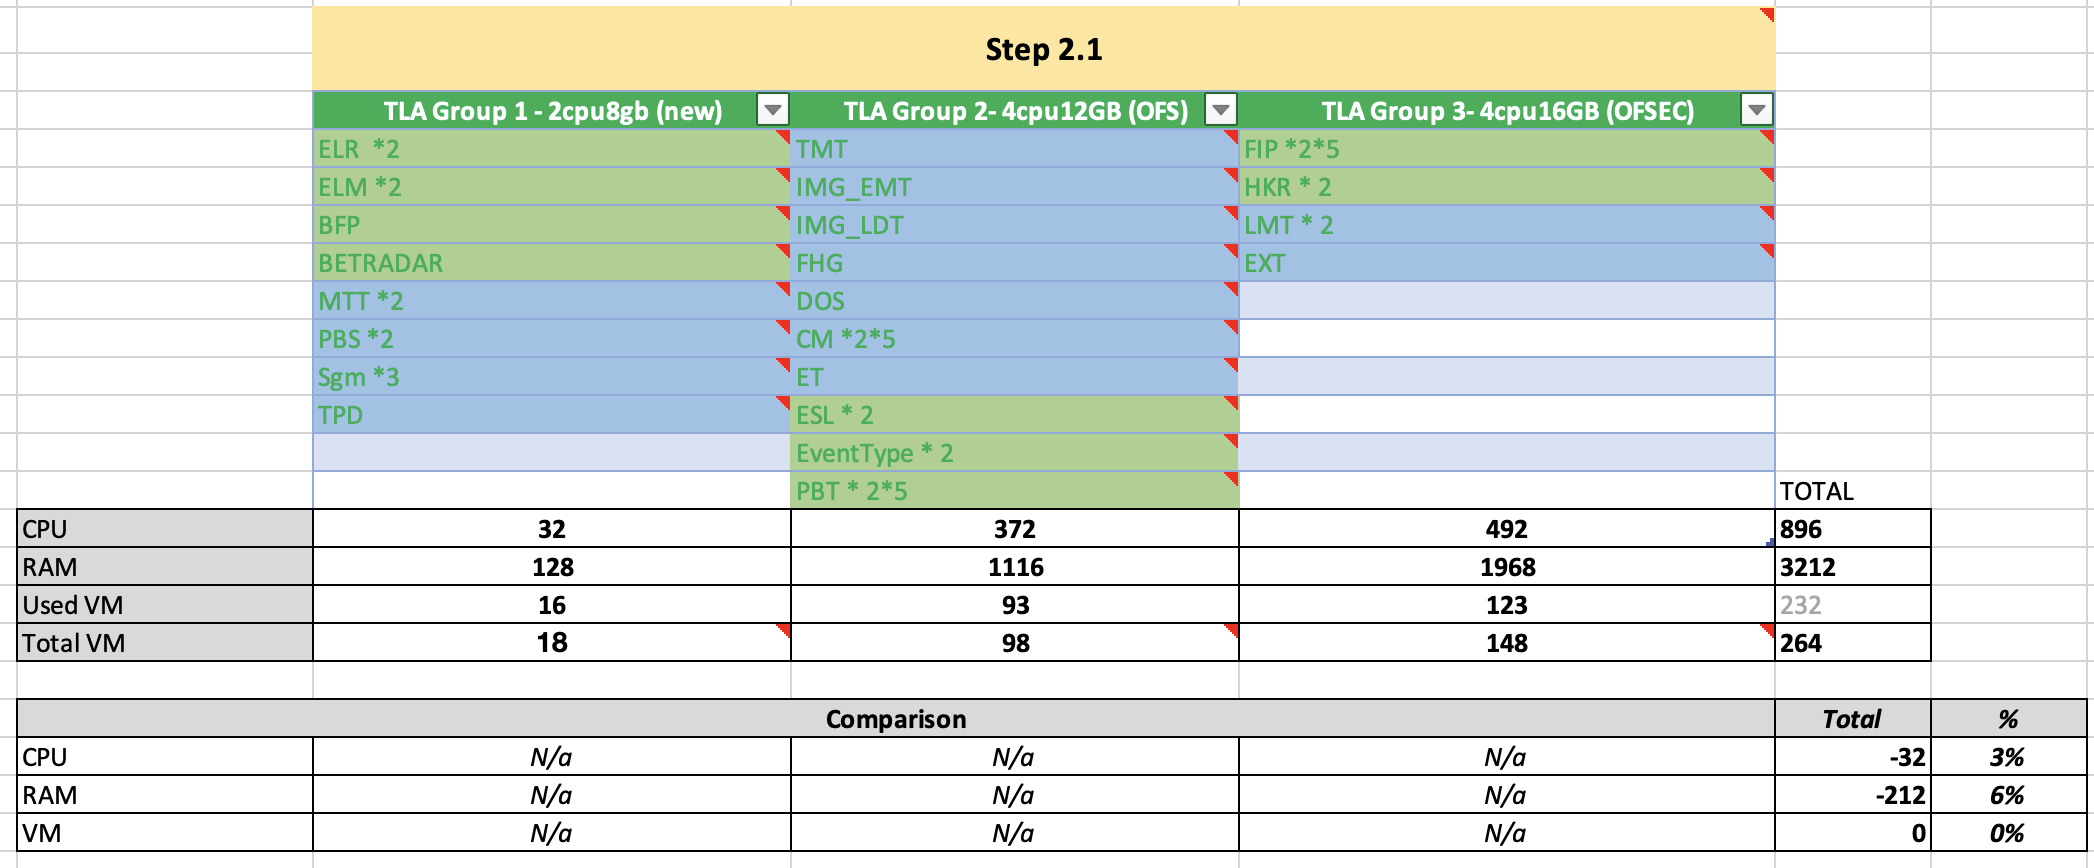
\includegraphics[scale=0.4]{media/content/analise/strat-2_1.png}}
  \caption{Processo de implantação - Passo 2.1}
  \label{strat-2_1}
\end{figure}

O terceiro, e último, passo, representando na Figura \ref{strat-3}, representa uma nova redução 
do \gls{flavour} de um dos \glspl{cluster}. Este passo é em todo semelhante ao primeiro, mas é
apenas necessário efetuar esta redução no segundo \gls{cluster}.

\begin{figure}[H]
  \centerline{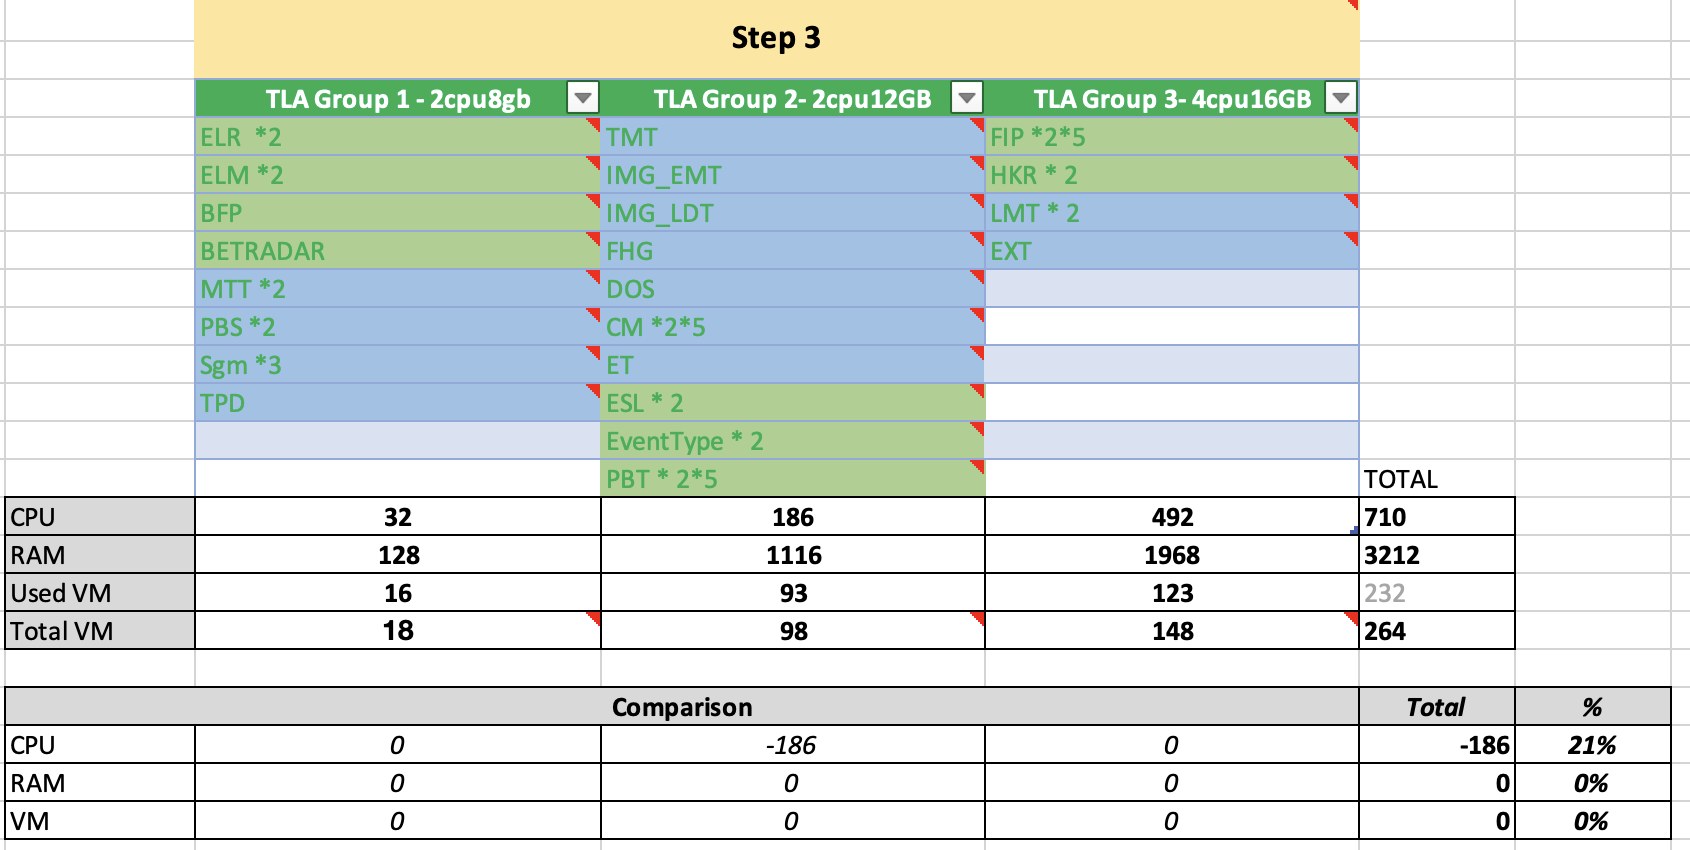
\includegraphics[scale=0.5]{media/content/analise/strat-3.png}}
  \caption{Processo de implantação - Passo 3}
  \label{strat-3}
\end{figure}

Após todo este processo a estrutura em que estão hospedadas as topologias encontra-se na forma
otimizada proposta e analisada anteriormente. Este processo sofre pequenas alterações entre
ambientes já que os \glspl{flavour} não são iguais entre estes. Além disso, durante este processo
tiveram que ser analisadas outras questões igualmente relevantes para garantir que esta migração
era possível como é o caso da capacidade de comunicação do \textit{Zookeeper}.

O \textit{Zookeeper} é utilizado por todos estes \glspl{cluster} para garantir a resiliência das 
topologias e, por consequência, poderia não ter a capacidade de comunicar com um \gls{cluster}
adicional. Após analisar esta questão com as equipas responsáveis pela infraestrutura foi 
determinado que esta questão representava um problema crítico para o desempenho do 
\textit{Zookeeper}, logo, a proposta foi aprovada.

